% !TeX spellcheck = ru_RU

\begin{figure}[h]
\begin{center}
    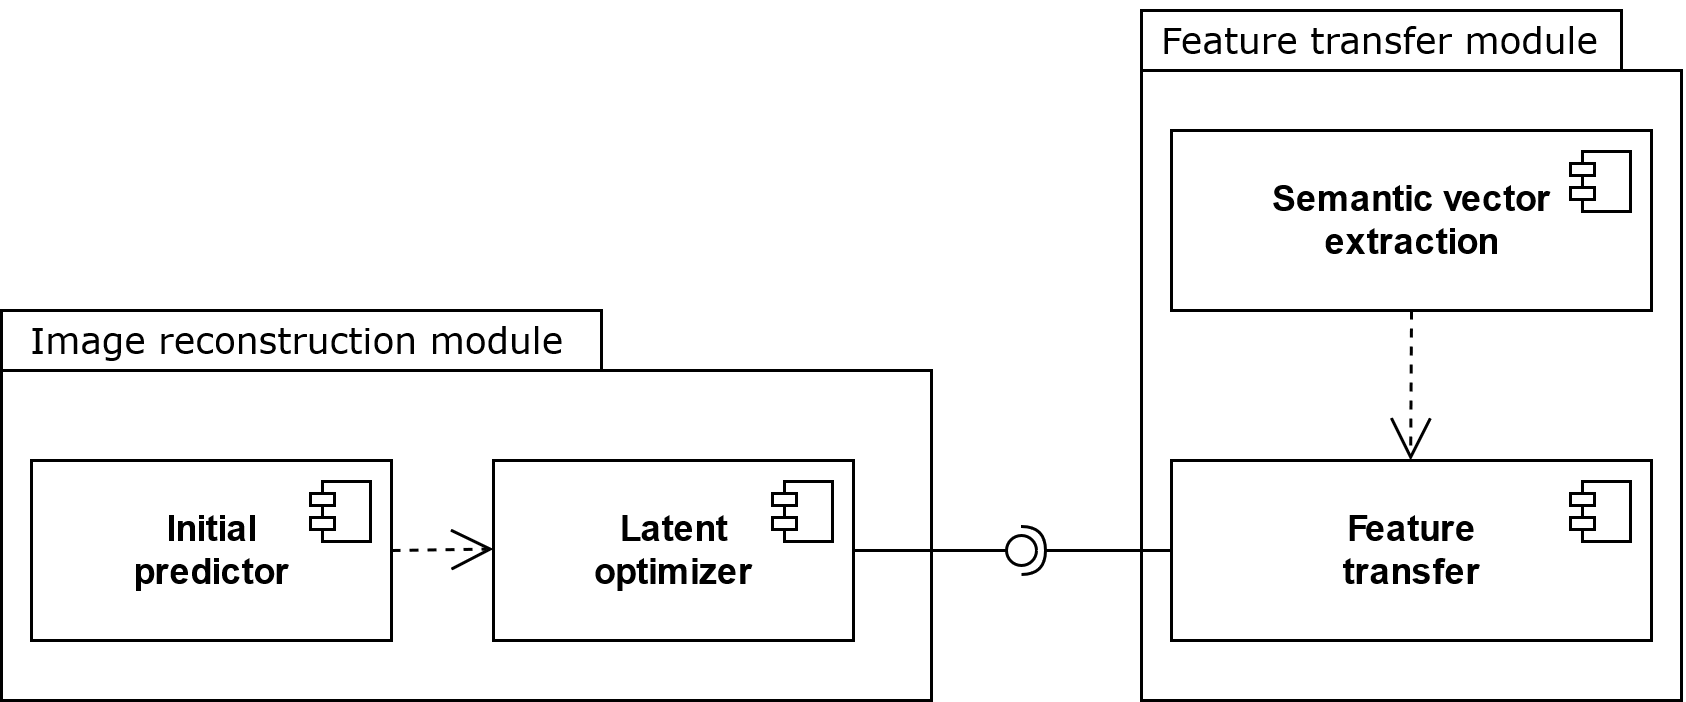
\includegraphics[width=0.9\textwidth]{Architecture_eng}
    \caption{Архитектура решения.}
    \label{fig:architecture}
\end{center}
\end{figure}

План:
\begin{enumerate}

\item
В рамках данной работы было разработано решение для семантического редактирования изображений, позволяющее редактировать изображения лиц в терминах высокоуровневых лицевых признаков, таких как положение головы, наличие улыбки и т.д.
По заданному бинарному лицевому признаку, это решение способно выделить семантический вектор в латентном пространстве генеративной состязательной сети, и произвести перенос информации об этом признаке с изображения-образца на целевое изображение.

\item
Решение состоит из двух функциональных частей: модуля реконструкции изображения (рис. \ref{fig:architecture}, \emph{Image reconstruction module}), и модуля семантического редактирования (рис. \ref{fig:architecture}, \emph{Feature transfer module}).

\item
Первый модуль осуществляет отображение входных изображений в латентное пространство имеющейся генеративной состязательной сети.
Он реализует гибридный алгоритм отображения, совмещающий обучение энкодера и латентную оптимизацию. 
Энкодер (компонент \emph{Initial predictor} на рис. \ref{fig:architecture}) используется для получения грубого начального приближения.
Затем это приближение итеративно улучшается с помощью латентной оптимизации (компонент \emph{Latent optimizer} на рис. \ref{fig:architecture}).

Такой алгоритм предостравляет пользователю гибкий контроль баланса между точностью реконструкции изображения и затраченным на обработку временем.

В качестве используемой архитектуры генеративной состязательной сети выбрана сеть StyleGAN, что позволет производить оптимизацию в расширенном латентном пространстве $\mathcal W+$.

\item
Второй модуль осуществляет семантическое редактирование изображений, реконструированных с помощью генеративной состязательной сети. 

Для нахождения семантического вектора, соответствующего редактируемому лицевому признаку, этим модулем реализуется алгоритм InterFaceGAN (компонент \emph{Semantic vector extraction} на рис. \ref{fig:architecture}).

Найденный семантический вектор передается в компонент, реализующий алгоритм переноса признака с изображения-образца на целевое изображение (\emph{Feature transfer} на рис. \ref{fig:architecture}).
Этот алгоритм основывается на алгоритме линейного сдвига латентного вектора, описанном в \cite{abdal2019image2stylegan}.
Для того, чтобы добиться более качественного переноса редактируемого признака и сохранения остальных признаков, производится модификация данного алгоритма, позволяющая производить нелинейный сдвиг в латентном пространстве сети.

Перенос признака сводится к минимизации функции потерь переноса
$$ 
\min_{\mathbf w} L(\mathbf w) = L_{feature}(\mathbf w, \mathbf w_{exemplar}) + \alpha~L_{identity}(\mathbf w, I_{real}),
$$
где член $L_{feature}$ осуществляет линейный сдвиг латентного вектора, найденного в ходе реконструкции входного изображения, в направлении, заданном семантическим вектором признака;  член $~L_{identity}$ осуществляет корректировку сдвига таким образом, чтобы он изменял лишь рассматриваемый признак, и, в частности, не затрагивал признаки, определяющие личность изображенного человека.

\end{enumerate}
